\section{Durchführung}
\label{durchfuehrung}

\begin{figure}
    \centering
    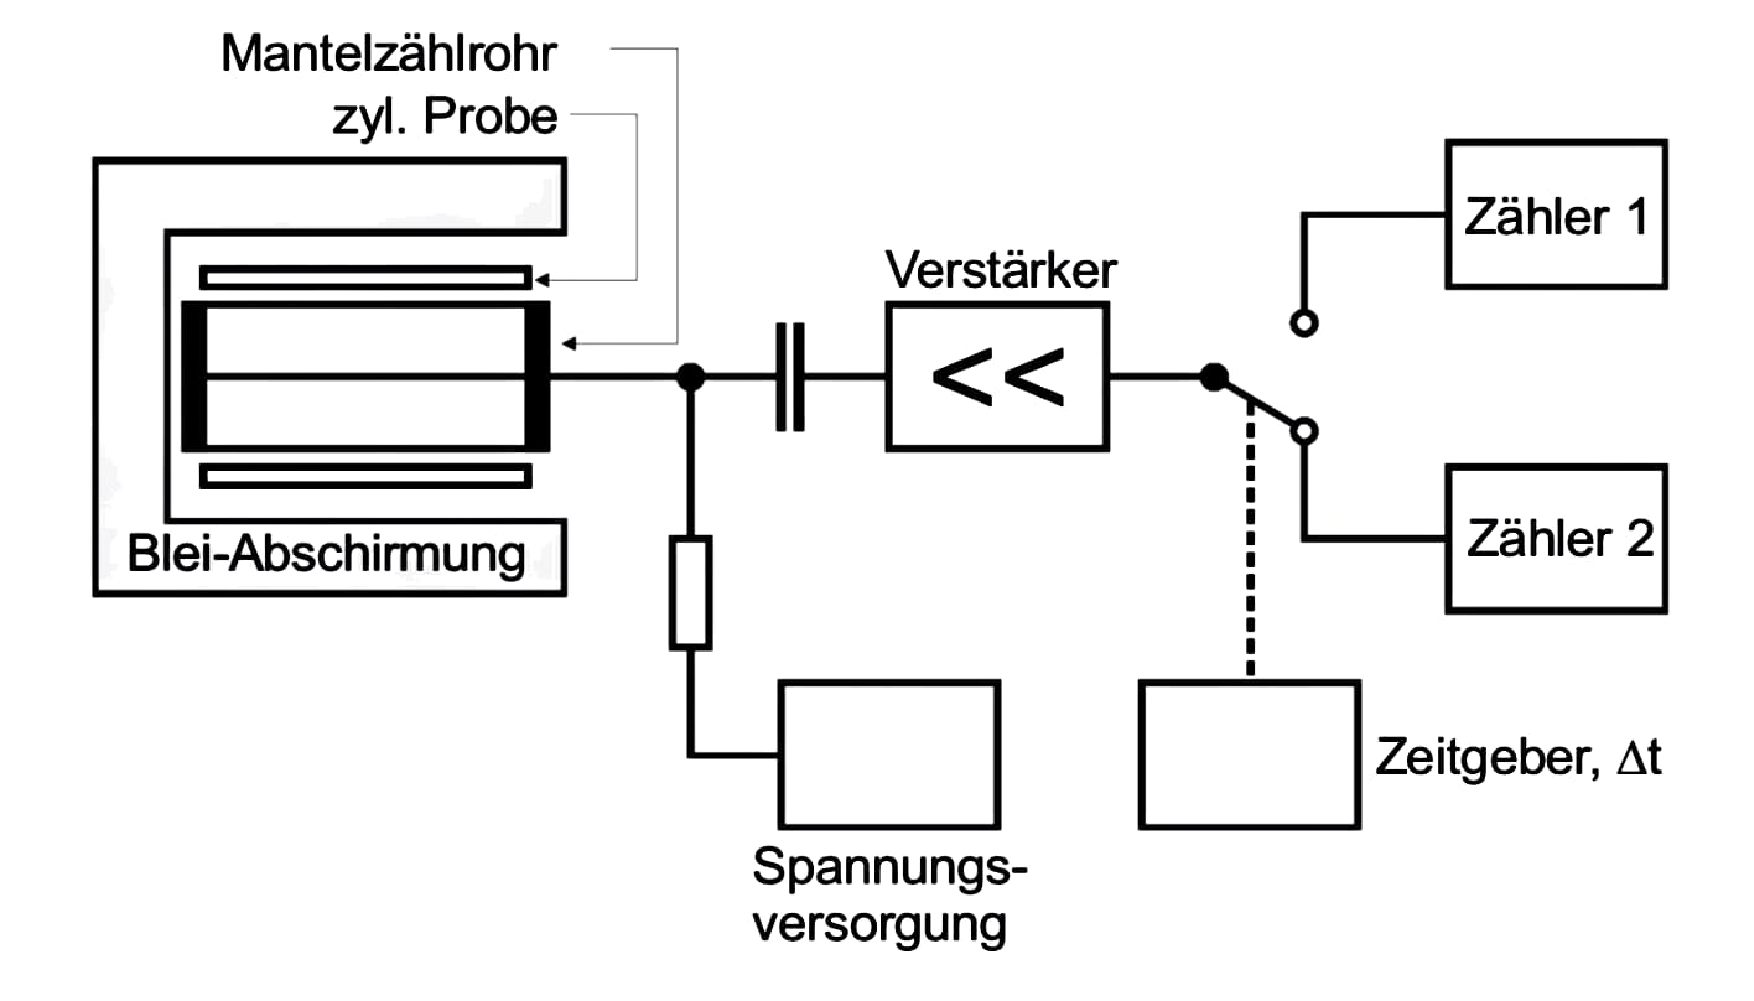
\includegraphics[scale = 0.35]{content/Aufbau2.pdf}
    \caption{Hier zu sehen ist eine Skizze zum Aufbau des Versuchs.}
    \label{fig:aufbau}
\end{figure}

Zunächst wird die Untergrundrate bestimmt. Da das Zählrohr auch ohne radioaktive Probe eine Zählrate registriert, muss dieser vorerst gemessen werden, um den Nulleffekt in die Berechnung einkalkulieren zu können. Es wird dabei die gemessene Zählrate von der Zählrate einer radioaktiven Probe subtrahiert, um nur letztere zu erhalten. Hier wird für das Zeitintervall der Messung 300 Sekunden gewählt, um dem wahren Wert \(N_U\) so nahe wie möglich zu kommen.\\
Danach wird die Halbwertszeit von Vanadium bestimmt. Für das Messintervall wird \(\Delta t\) = 30 Sekunden gewählt. Die Vanadiumprobe wird, nach dem Entnehmen aus der Neutronenquelle, in das Geiger-Müller-Zählrohr eingeführt und die Messung gestartet.\\
Das Prozedere wird für die Bestimmung der Halbwertszeit von Rhodium wiederholt, wobei \(\Delta t\) = 15 Sekunden gewählt wird.